\documentclass[notes,11pt, aspectratio=169]{beamer}

\usepackage{pgfpages}
\setbeameroption{hide notes} % Only slide

\usepackage{helvet}
\usepackage[default]{lato}
\usepackage{array}
\usepackage{tgbonum}

\usepackage{tikz}
\usepackage{verbatim}
\setbeamertemplate{note page}{\pagecolor{yellow!5}\insertnote}
\usetikzlibrary{positioning}
\usetikzlibrary{calc}
\usetikzlibrary{arrows}
\usetikzlibrary{arrows.meta}
\usetikzlibrary{decorations.markings}
\usetikzlibrary{decorations.pathreplacing}
\usetikzlibrary{shapes.misc}
\usetikzlibrary{shapes.geometric}
\usetikzlibrary{matrix,shapes,arrows,fit,tikzmark}
\usepackage{amsmath}
\usepackage{amssymb}
\usepackage{mathtools}
\usepackage{bm}
\usepackage{mathpazo}
\usepackage{hyperref}
\usepackage{lipsum}
\usepackage{multimedia}
\usepackage{graphicx}
\usepackage{multirow}
\usepackage{dcolumn}
\usepackage{bbm}
\usepackage{pgfplots}
\pgfplotsset{compat=1.18}
\usepackage{listings}
\newcolumntype{d}[0]{D{.}{.}{5}}

\usepackage{changepage}
\usepackage{appendixnumberbeamer}
\newcommand{\beginbackup}{
   \newcounter{framenumbervorappendix}
   \setcounter{framenumbervorappendix}{\value{framenumber}}
   \setbeamertemplate{footline}
   {
     \leavevmode%
     \hline
     box{%
       \begin{beamercolorbox}[wd=\paperwidth,ht=2.25ex,dp=1ex,right]{footlinecolor}%
       \end{beamercolorbox}}%
     \vskip0pt%
   }
 }
\newcommand{\backupend}{
   \addtocounter{framenumbervorappendix}{-\value{framenumber}}
   \addtocounter{framenumber}{\value{framenumbervorappendix}}
}

\usepackage[space]{grffile}
\usepackage{booktabs}
\newcommand\independent{\protect\mathpalette{\protect\independenT}{\perp}}
\def\independenT#1#2{\mathrel{\rlap{$#1#2$}\mkern2mu{#1#2}}}
\DeclareMathOperator{\Supp}{Supp}
\DeclareMathOperator*{\argmin}{arg\,min}

% Colors
\definecolor{blue}{RGB}{0,114,178}
\definecolor{red}{RGB}{213,94,0}
\definecolor{yellow}{RGB}{240,228,66}
\definecolor{green}{RGB}{0,158,115}

\hypersetup{
  colorlinks=true,
  linkbordercolor = {white},
  linkcolor = {blue}
}

\definecolor{MyBackground}{RGB}{255,253,218}

\newenvironment{transitionframe}{
  \setbeamercolor{background canvas}{bg=yellow}
  \begin{frame}}{
    \end{frame}
}

\setbeamercolor{frametitle}{fg=blue}
\setbeamercolor{title}{fg=black}
\setbeamertemplate{footline}[frame number]
\setbeamertemplate{navigation symbols}{}
\setbeamertemplate{itemize items}{-}
\setbeamercolor{itemize item}{fg=blue}
\setbeamercolor{itemize subitem}{fg=blue}
\setbeamercolor{enumerate item}{fg=blue}
\setbeamercolor{enumerate subitem}{fg=blue}
\setbeamercolor{button}{bg=MyBackground,fg=blue,}

\setbeamercolor{section in toc}{fg=blue}
\setbeamercolor{subsection in toc}{fg=red}
\setbeamersize{text margin left=1em,text margin right=1em}

\newenvironment{wideitemize}{\itemize\addtolength{\itemsep}{10pt}}{\enditemize}

% Code listing style
\lstset{
    language=Python,
    basicstyle=\ttfamily\scriptsize,
    keywordstyle=\color{blue}\bfseries,
    stringstyle=\color{red!70!black},
    commentstyle=\color{green!50!black}\itshape,
    numbers=left,
    numberstyle=\tiny\color{gray},
    numbersep=5pt,
    frame=single,
    breaklines=true,
    backgroundcolor=\color{gray!5},
    showstringspaces=false,
    tabsize=4
}

% Math shortcuts
\newcommand{\vx}{\mathbf{x}}
\newcommand{\vw}{\mathbf{w}}
\newcommand{\vb}{\mathbf{b}}
\newcommand{\vh}{\mathbf{h}}
\newcommand{\vy}{\mathbf{y}}
\newcommand{\vz}{\mathbf{z}}
\newcommand{\va}{\mathbf{a}}
\newcommand{\vW}{\mathbf{W}}
\newcommand{\vZ}{\mathbf{Z}}
\newcommand{\R}{\mathbb{R}}
\newcommand{\E}{\mathbb{E}}
\newcommand{\pd}[2]{\frac{\partial #1}{\partial #2}}


\title[]{\textcolor{blue}{Advanced Methods in Deep Learning}\\ \textcolor{black}{\normalsize Lecture 2: Non-linearities, Loss Functions, Backpropagation \& Gradient Descent}}
\author[Quispe]{}
\institute[MECA]{\small{Alexander Quispe Rojas \\ Universidad del Pac\'ifico -- MECA  \\ aw.quispero@up.edu.pe \quad aquisper@caltech.edu}}
\date{April 17, 2026}


\begin{document}

%%% TIKZ STUFF
\tikzset{
        every picture/.style={remember picture,baseline},
        every node/.style={anchor=base,align=center,outer sep=1.5pt},
        every path/.style={thick},
        }
\tikzstyle{every picture}+=[remember picture]
\tikzstyle{mybox} =[draw=black, very thick, rectangle, inner sep=10pt, inner ysep=20pt]
\tikzstyle{fancytitle} =[draw=black,fill=red, text=white]
%%%% END TIKZ STUFF

% ============================================================
% Title Slide
% ============================================================
\begin{frame}
\maketitle
\end{frame}

\begin{frame}
\frametitle{Today's Roadmap}
\tableofcontents
\end{frame}


% ============================================================
\section{Recap and Activation Functions Deep Dive}
% ============================================================

\begin{transitionframe}
\begin{center}
{\Huge \textbf{Recap \& Activation Functions}}
\end{center}
\end{transitionframe}

% ---- Recap ----
\begin{frame}
\frametitle{Recap from Lecture 1}

\textbf{What we learned:}
\begin{wideitemize}
    \item A neural network computes: $\vh^{(l)} = \sigma(\vW^{(l)}\vh^{(l-1)} + \vb^{(l)})$.
    \item The \textbf{forward pass} maps input $\vx$ to prediction $\hat{y}$.
    \item We need a \textbf{loss function} $\mathcal{L}$ to measure how bad our prediction is.
    \item We use \textbf{gradient descent} to update parameters: $\vw \leftarrow \vw - \alpha \nabla_{\vw}\mathcal{L}$.
\end{wideitemize}

\vspace{10pt}
\textbf{Today's question:}
\begin{center}
\textcolor{red}{\Large How do we compute $\nabla_{\vw}\mathcal{L}$ efficiently for a deep network?}
\end{center}

\vspace{6pt}
\textbf{Answer:} The \textbf{backpropagation} algorithm --- a systematic application of the chain rule.
\end{frame}

% ---- Activation Functions Revisited ----
\begin{frame}
\frametitle{Activation Functions: Derivatives Matter}

To do backpropagation, we need the \textbf{derivative} of each activation function.

\vspace{4pt}
\renewcommand{\arraystretch}{1.6}
\begin{center}
{\small
\begin{tabular}{llll}
\toprule
\textbf{Name} & \textbf{$\sigma(z)$} & \textbf{$\sigma'(z)$} & \textbf{Range} \\
\midrule
Sigmoid & $\frac{1}{1+e^{-z}}$ & $\sigma(z)(1 - \sigma(z))$ & $(0, 1)$ \\[3pt]
Tanh & $\frac{e^z - e^{-z}}{e^z + e^{-z}}$ & $1 - \tanh^2(z)$ & $(-1, 1)$ \\[3pt]
ReLU & $\max(0, z)$ & $1$ if $z > 0$; $0$ if $z < 0$ & $[0, \infty)$ \\[3pt]
Leaky ReLU & $\max(\alpha z, z)$ & $1$ if $z > 0$; $\alpha$ if $z < 0$ & $(-\infty, \infty)$ \\
\bottomrule
\end{tabular}
}
\end{center}
\end{frame}

% ---- Sigmoid Derivative ----
\begin{frame}
\frametitle{Deriving the Sigmoid Derivative}

Let $\sigma(z) = \frac{1}{1 + e^{-z}} = (1 + e^{-z})^{-1}$. Apply the chain rule:

\vspace{2pt}
\textbf{Step 1:}
$\sigma'(z) = -(1 + e^{-z})^{-2} \cdot (-e^{-z}) = \frac{e^{-z}}{(1 + e^{-z})^2}$

\vspace{4pt}
\textbf{Step 2:} Rewrite in terms of $\sigma(z)$:
\[
    \sigma'(z) = \frac{1}{1+e^{-z}} \cdot \frac{e^{-z}}{1+e^{-z}} = \sigma(z) \cdot \frac{(1 + e^{-z}) - 1}{1+e^{-z}} = \sigma(z)(1 - \sigma(z))
\]

\begin{tikzpicture}
\node [mybox] (box){%
    \begin{minipage}{0.93\textwidth}
    \vspace{-6pt}
    \[
        \boxed{\sigma'(z) = \sigma(z)\big(1 - \sigma(z)\big)}
    \]
    \vspace{-8pt}
    \textbf{Note:} Max value $\sigma'(0) = 0.25$. This causes the \textcolor{red}{vanishing gradient problem}.
    \end{minipage}
};
\node[fancytitle, right=10pt] at (box.north west) {Result};
\end{tikzpicture}
\end{frame}

% ---- Vanishing Gradient ----
\begin{frame}
\frametitle{The Vanishing Gradient Problem}

\begin{columns}[T]
\begin{column}{0.48\textwidth}
\textbf{Sigmoid derivative} peaks at $0.25$:

\begin{center}
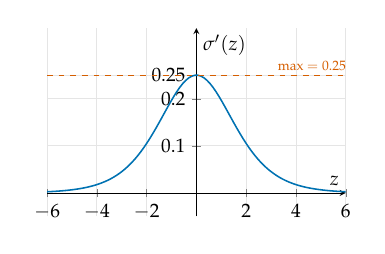
\begin{tikzpicture}[scale=0.7]
    \begin{axis}[
        xlabel={$z$}, ylabel={$\sigma'(z)$},
        xmin=-6, xmax=6, ymin=-0.05, ymax=0.35,
        width=7cm, height=5cm,
        axis lines=middle,
        grid=major, grid style={gray!20},
        ytick={0, 0.1, 0.2, 0.25},
    ]
    \addplot[thick, blue, domain=-6:6, samples=100] {exp(-x)/((1+exp(-x))^2)};
    \draw[dashed, red] (axis cs:-6,0.25) -- (axis cs:6,0.25);
    \node[right, font=\scriptsize, text=red] at (axis cs:3, 0.27) {max $= 0.25$};
    \end{axis}
\end{tikzpicture}
\end{center}
\end{column}

\begin{column}{0.48\textwidth}
\textbf{Problem for deep networks:}

With $L$ layers of sigmoid, the gradient at layer 1 involves:
\[
    \pd{\mathcal{L}}{\vW^{(1)}} \propto \prod_{l=1}^{L} \sigma'(z^{(l)})
\]

\vspace{4pt}
Since $\sigma'(z) \leq 0.25$:
\[
    \prod_{l=1}^{L} 0.25 = 0.25^L
\]

\vspace{4pt}
For $L = 10$: $0.25^{10} \approx 10^{-6}$

\vspace{6pt}
\textcolor{red}{\textbf{Gradients vanish exponentially with depth!}}
\end{column}
\end{columns}

\vspace{8pt}
\textbf{Solution:} Use \textbf{ReLU}, where $\sigma'(z) = 1$ for $z > 0$. No vanishing gradient!
\end{frame}

% ---- ReLU advantages ----
\begin{frame}
\frametitle{Why ReLU Dominates}

\begin{columns}[T]
\begin{column}{0.48\textwidth}
\begin{center}
\textcolor{blue}{\textbf{ReLU:}} $\sigma(z) = \max(0, z)$

\begin{tikzpicture}[scale=0.65]
    \begin{axis}[
        width=6cm, height=5cm,
        xmin=-4, xmax=4, ymin=-0.5, ymax=4,
        axis lines=middle, ticks=none,
        xlabel={$z$}, ylabel={$\sigma(z)$}
    ]
    \addplot[thick, red, domain=-4:0] {0};
    \addplot[thick, red, domain=0:4] {x};
    \end{axis}
\end{tikzpicture}
\end{center}

\begin{wideitemize}
    \item Derivative $= 1$ for $z > 0$: no vanishing gradient.
    \item Computationally cheap.
    \item Sparse activation (many neurons output 0).
\end{wideitemize}
\end{column}

\begin{column}{0.48\textwidth}
\begin{center}
\textcolor{blue}{\textbf{ReLU derivative:}}

\begin{tikzpicture}[scale=0.65]
    \begin{axis}[
        width=6cm, height=5cm,
        xmin=-4, xmax=4, ymin=-0.5, ymax=1.5,
        axis lines=middle, ticks=none,
        xlabel={$z$}, ylabel={$\sigma'(z)$}
    ]
    \addplot[thick, blue, domain=-4:-0.01] {0};
    \addplot[thick, blue, domain=0.01:4] {1};
    \addplot[only marks, mark=*, mark size=2pt, blue] coordinates {(0,0)};
    \end{axis}
\end{tikzpicture}
\end{center}

\textcolor{red}{\textbf{Problem:}} ``Dead ReLU'' --- if $z < 0$ always, the neuron never updates.

\vspace{6pt}
\textbf{Fix:} Leaky ReLU ($\alpha = 0.01$), ELU, GELU.
\end{column}
\end{columns}
\end{frame}

% ---- Softmax ----
\begin{frame}
\frametitle{Softmax: From Binary to Multi-class Classification}

For $K$ classes, we need a probability distribution over classes.

\begin{tikzpicture}
\node [mybox] (box){%
    \begin{minipage}{0.93\textwidth}
    Given logits $z_1, z_2, \ldots, z_K$ (raw outputs of the network), the \textbf{softmax} function computes:
    \[
        p(y = k | \vx) = \text{softmax}(z_k) = \frac{e^{z_k}}{\sum_{j=1}^{K} e^{z_j}} \qquad \text{for } k = 1, \ldots, K
    \]
    \end{minipage}
};
\node[fancytitle, right=10pt] at (box.north west) {Softmax Function};
\end{tikzpicture}

\vspace{6pt}
\textbf{Properties:}
\begin{wideitemize}
    \item $\sum_{k=1}^{K} p(y = k | \vx) = 1$ \quad (valid probability distribution).
    \item $p(y = k | \vx) > 0$ for all $k$ \quad (always positive).
    \item Larger $z_k$ $\Rightarrow$ higher probability for class $k$.
    \item When $K = 2$: softmax reduces to the sigmoid function.
\end{wideitemize}
\end{frame}

% ---- Softmax Example ----
\begin{frame}
\frametitle{Softmax: Numerical Example}

\textbf{Network output (logits)} for $K = 3$ classes:
\[
    \vz = \begin{pmatrix} z_1 \\ z_2 \\ z_3 \end{pmatrix} = \begin{pmatrix} 2.0 \\ 1.0 \\ 0.1 \end{pmatrix}
\]

\textbf{Step 1:} Compute exponentials:
\[
    e^{z_1} = e^{2.0} = 7.389, \quad e^{z_2} = e^{1.0} = 2.718, \quad e^{z_3} = e^{0.1} = 1.105
\]

\textbf{Step 2:} Sum of exponentials:
\[
    \sum_{j=1}^{3} e^{z_j} = 7.389 + 2.718 + 1.105 = 11.212
\]

\textbf{Step 3:} Normalize:
\[
    p_1 = \frac{7.389}{11.212} = \textcolor{red}{0.659}, \quad p_2 = \frac{2.718}{11.212} = 0.242, \quad p_3 = \frac{1.105}{11.212} = 0.099
\]

\vspace{4pt}
\textbf{Prediction:} class 1 with probability 65.9\%. \quad Check: $0.659 + 0.242 + 0.099 = 1.0$ \; $\checkmark$
\end{frame}


% ============================================================
\section{Loss Functions in Detail}
% ============================================================

\begin{transitionframe}
\begin{center}
{\Huge \textbf{Loss Functions in Detail}}
\end{center}
\end{transitionframe}

% ---- Loss Functions Overview ----
\begin{frame}
\frametitle{Loss Functions: Overview}

The loss function $\mathcal{L}$ measures how far our prediction $\hat{y}$ is from the truth $y$.

\vspace{8pt}
\renewcommand{\arraystretch}{1.6}
\begin{center}
\begin{tabular}{llll}
\toprule
\textbf{Task} & \textbf{Loss} & \textbf{Formula} & \textbf{Output activation} \\
\midrule
Regression & MSE & $\frac{1}{N}\sum(y_i - \hat{y}_i)^2$ & None (linear) \\
Binary classif.\ & BCE & $-\frac{1}{N}\sum[y\log\hat{y} + (1-y)\log(1-\hat{y})]$ & Sigmoid \\
Multi-class & CE & $-\frac{1}{N}\sum\sum y_{ik}\log \hat{y}_{ik}$ & Softmax \\
\bottomrule
\end{tabular}
\end{center}

\vspace{8pt}
\textbf{Key principle:} the choice of loss function depends on the task. The loss determines what the network optimizes for.
\end{frame}

% ---- MSE Gradient ----
\begin{frame}
\frametitle{MSE Loss: Gradient Derivation}

\textbf{Loss for one sample:} $\ell = (y - \hat{y})^2$ where $\hat{y} = f(\vx; \theta)$.

\vspace{6pt}
\textbf{Gradient with respect to the prediction:}
\[
    \pd{\ell}{\hat{y}} = \pd{}{\hat{y}}(y - \hat{y})^2 = 2(y - \hat{y}) \cdot (-1) = \textcolor{red}{-2(y - \hat{y})}
\]

\vspace{4pt}
\textbf{Average over $N$ samples:}
\[
    \pd{\mathcal{L}}{\hat{y}_i} = -\frac{2}{N}(y_i - \hat{y}_i)
\]

\vspace{6pt}
\textbf{Interpretation:}
\begin{wideitemize}
    \item The gradient is proportional to the \textbf{error} $(y_i - \hat{y}_i)$.
    \item Large errors produce large gradients $\Rightarrow$ faster learning.
    \item This is the \textbf{starting point} of backpropagation: we first compute $\pd{\mathcal{L}}{\hat{y}}$, then propagate backward.
\end{wideitemize}
\end{frame}

% ---- BCE Derivation ----
\begin{frame}
\frametitle{Binary Cross-Entropy: Derivation from MLE}

Assume $y \in \{0, 1\}$ and model predicts $\hat{y} = p(y=1|\vx)$. Likelihood of one sample:
$p(y | \vx) = \hat{y}^{y}(1 - \hat{y})^{1-y}$.

\vspace{2pt}
\textbf{Log-likelihood} $\to$ \textbf{Negative log-likelihood} (= BCE):
\[
    \ell = -\big[y \log \hat{y} + (1-y) \log(1 - \hat{y})\big]
\]

\textbf{Gradient w.r.t.\ $\hat{y}$:}
\[
    \pd{\ell}{\hat{y}} = -\frac{y}{\hat{y}} + \frac{1-y}{1-\hat{y}} = \frac{\hat{y} - y}{\hat{y}(1-\hat{y})}
\]

\textbf{Gradient w.r.t.\ logit $z$} (where $\hat{y} = \sigma(z)$, $\sigma' = \sigma(1-\sigma)$):
\[
    \pd{\ell}{z} = \pd{\ell}{\hat{y}} \cdot \sigma'(z) = \frac{\hat{y} - y}{\hat{y}(1-\hat{y})} \cdot \hat{y}(1-\hat{y}) = \textcolor{red}{\hat{y} - y}
\]
\end{frame}

% ---- BCE Gradient Beauty ----
\begin{frame}
\frametitle{The Beautiful Cancellation: BCE + Sigmoid}

\begin{tikzpicture}
\node [mybox] (box){%
    \begin{minipage}{0.93\textwidth}
    \[
        \pd{\ell}{z} = \sigma(z) - y = \hat{y} - y
    \]
    The gradient of the BCE loss with respect to the logit $z$ is simply $\hat{y} - y$.
    \end{minipage}
};
\node[fancytitle, right=10pt] at (box.north west) {Key Result};
\end{tikzpicture}

\vspace{8pt}
\textbf{Why is this beautiful?}
\begin{wideitemize}
    \item No $\sigma'(z) = \sigma(z)(1-\sigma(z))$ term in the gradient!
    \item Even when $\sigma'(z)$ is tiny (saturated sigmoid), the gradient is still large if the prediction is wrong.
    \item \textbf{This is not a coincidence:} BCE was designed precisely because it pairs well with sigmoid.
    \item Compare: MSE + sigmoid $\Rightarrow$ $\pd{\ell}{z} = -2(y - \hat{y})\sigma'(z)$ \quad (vanishes when saturated!).
\end{wideitemize}

\vspace{6pt}
\textbf{Lesson:} \textcolor{red}{Always pair the right loss with the right activation.}
\end{frame}

% ---- Categorical Cross-Entropy ----
\begin{frame}
\frametitle{Categorical Cross-Entropy Loss}

For $K$-class classification with one-hot encoding $\vy = (y_1, \ldots, y_K)$:

\begin{tikzpicture}
\node [mybox] (box){%
    \begin{minipage}{0.93\textwidth}
    \[
        \mathcal{L} = -\sum_{k=1}^{K} y_k \log \hat{y}_k = -\log \hat{y}_c
    \]
    where $c$ is the true class (since only $y_c = 1$, all other $y_k = 0$).
    \end{minipage}
};
\node[fancytitle, right=10pt] at (box.north west) {Categorical Cross-Entropy};
\end{tikzpicture}

\vspace{6pt}
\textbf{Example:} True class $= 2$ (i.e., $\vy = (0, 1, 0)$), predictions $\hat{\vy} = (0.1, 0.7, 0.2)$:
\[
    \mathcal{L} = -(0 \cdot \log 0.1 + 1 \cdot \log 0.7 + 0 \cdot \log 0.2) = -\log(0.7) = 0.357
\]

\vspace{4pt}
If predictions were $\hat{\vy} = (0.1, 0.95, 0.05)$:
\[
    \mathcal{L} = -\log(0.95) = 0.051 \quad \text{(much lower --- better prediction)}
\]

\vspace{6pt}
\textbf{Interpretation:} The loss only depends on the \textbf{predicted probability for the correct class}.
\end{frame}

% ---- Softmax Jacobian ----
\begin{frame}
\frametitle{Softmax + Cross-Entropy: Gradient (Step 1)}

Let $\hat{y}_k = \text{softmax}(z_k) = \frac{e^{z_k}}{\sum_j e^{z_j}}$ and $\mathcal{L} = -\sum_k y_k \log \hat{y}_k$.

\vspace{6pt}
\textbf{We want:} $\pd{\mathcal{L}}{z_i}$ for each logit $z_i$. First, compute the \textbf{Jacobian of softmax}:

\vspace{4pt}
\textbf{Case $i = k$:}
\[
    \pd{\hat{y}_k}{z_k} = \frac{e^{z_k}\sum_j e^{z_j} - e^{z_k} \cdot e^{z_k}}{(\sum_j e^{z_j})^2} = \hat{y}_k - \hat{y}_k^2 = \hat{y}_k(1 - \hat{y}_k)
\]

\textbf{Case $i \neq k$:}
\[
    \pd{\hat{y}_k}{z_i} = \frac{0 - e^{z_k} \cdot e^{z_i}}{(\sum_j e^{z_j})^2} = -\hat{y}_k \hat{y}_i
\]

\vspace{6pt}
\textbf{Compact form:} \quad $\pd{\hat{y}_k}{z_i} = \hat{y}_k(\delta_{ik} - \hat{y}_i)$ \quad where $\delta_{ik}$ is the Kronecker delta.
\end{frame}

% ---- Softmax + CE Gradient Step 2 ----
\begin{frame}
\frametitle{Softmax + Cross-Entropy: Gradient (Step 2)}

\textbf{Step 2:} Apply chain rule with $\mathcal{L} = -\sum_k y_k \log \hat{y}_k$:
\[
    \pd{\mathcal{L}}{z_i} = \sum_{k=1}^{K} \pd{\mathcal{L}}{\hat{y}_k} \cdot \pd{\hat{y}_k}{z_i} = -\sum_{k=1}^{K} \frac{y_k}{\hat{y}_k} \cdot \hat{y}_k(\delta_{ik} - \hat{y}_i)
\]

\vspace{4pt}
\textbf{Simplify:}
\[
    = -\sum_{k} y_k(\delta_{ik} - \hat{y}_i) = -y_i + \hat{y}_i \underbrace{\sum_{k} y_k}_{=1} = \hat{y}_i - y_i
\]

\vspace{6pt}
\begin{tikzpicture}
\node [mybox] (box){%
    \begin{minipage}{0.93\textwidth}
    \vspace{-6pt}
    \[
        \boxed{\pd{\mathcal{L}}{z_i} = \hat{y}_i - y_i \qquad \text{(prediction minus truth)}}
    \]
    \vspace{-6pt}
    Same result as BCE + sigmoid! This elegant cancellation is by design.
    \end{minipage}
};
\node[fancytitle, right=10pt] at (box.north west) {Key Result};
\end{tikzpicture}
\end{frame}


% ============================================================
\section{The Chain Rule}
% ============================================================

\begin{transitionframe}
\begin{center}
{\Huge \textbf{The Chain Rule}}
\end{center}
\end{transitionframe}

% ---- Single Variable Chain Rule ----
\begin{frame}
\frametitle{The Chain Rule: Single Variable}

If $y = f(u)$ and $u = g(x)$, then:
\[
    \frac{dy}{dx} = \frac{dy}{du} \cdot \frac{du}{dx}
\]

\vspace{6pt}
\textbf{Example:} Let $y = (3x + 2)^2$.
\begin{itemize}
    \item Let $u = 3x + 2$, so $y = u^2$.
    \item $\frac{dy}{du} = 2u = 2(3x+2)$.
    \item $\frac{du}{dx} = 3$.
    \item $\frac{dy}{dx} = 2(3x+2) \cdot 3 = 6(3x+2)$.
\end{itemize}

\vspace{8pt}
\textbf{Longer chains:} If $y = f(g(h(x)))$:
\[
    \frac{dy}{dx} = \frac{dy}{dg} \cdot \frac{dg}{dh} \cdot \frac{dh}{dx}
\]

\vspace{4pt}
\textcolor{red}{\textbf{This is exactly what happens in a neural network:} each layer is a function composition.}
\end{frame}

% ---- Multivariate Chain Rule ----
\begin{frame}
\frametitle{The Chain Rule: Multiple Variables}

If $\mathcal{L} = f(y_1, y_2)$ where $y_1 = g_1(x)$ and $y_2 = g_2(x)$:
\[
    \pd{\mathcal{L}}{x} = \pd{\mathcal{L}}{y_1}\pd{y_1}{x} + \pd{\mathcal{L}}{y_2}\pd{y_2}{x}
\]

\vspace{4pt}
\textbf{In general,} if $\mathcal{L}$ depends on $x$ through $y_1, y_2, \ldots, y_m$:
\[
    \pd{\mathcal{L}}{x} = \sum_{j=1}^{m} \pd{\mathcal{L}}{y_j}\pd{y_j}{x}
\]

\vspace{8pt}
\textbf{Example (relevant to neural networks):}

A weight $w_{13}^{(1)}$ in layer 1 affects multiple hidden neurons, which all affect the loss:
\[
    \pd{\mathcal{L}}{w_{13}^{(1)}} = \sum_{j} \pd{\mathcal{L}}{h_j^{(2)}} \cdot \pd{h_j^{(2)}}{w_{13}^{(1)}}
\]

\vspace{4pt}
\textcolor{red}{We need to sum contributions from all paths through the network.}
\end{frame}

% ---- Computational Graph ----
\begin{frame}
\frametitle{Computational Graphs}

A \textbf{computational graph} represents a function as a sequence of operations.

\vspace{6pt}
\textbf{Example:} $\mathcal{L} = (y - \sigma(wx + b))^2$

\begin{center}
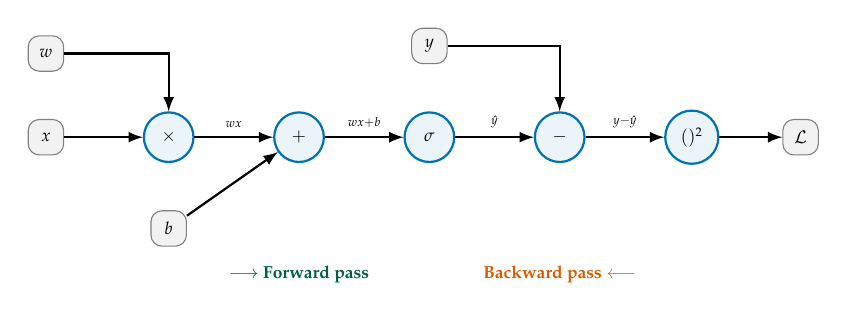
\begin{tikzpicture}[
    node distance=1.1cm,
    op/.style={circle, draw=blue, thick, minimum size=0.7cm, fill=blue!8, font=\scriptsize},
    var/.style={rectangle, draw=gray, rounded corners, minimum size=0.5cm, fill=gray!10, font=\scriptsize},
    >=latex,
    scale=0.9, every node/.style={scale=0.9}
]
    \node[var] (x) {$x$};
    \node[var, above=0.6cm of x] (w) {$w$};
    \node[op, right=1cm of x] (mul) {$\times$};
    \node[var, below=0.6cm of mul] (b) {$b$};
    \node[op, right=1cm of mul] (add) {$+$};
    \node[op, right=1cm of add] (sig) {$\sigma$};
    \node[var, above=0.6cm of sig] (y) {$y$};
    \node[op, right=1cm of sig] (sub) {$-$};
    \node[op, right=1cm of sub] (sq) {$()^2$};
    \node[var, right=0.8cm of sq] (L) {$\mathcal{L}$};

    \draw[->, thick] (x) -- (mul);
    \draw[->, thick] (w) -| (mul);
    \draw[->, thick] (mul) -- node[above, font=\tiny] {$wx$} (add);
    \draw[->, thick] (b) -- (add);
    \draw[->, thick] (add) -- node[above, font=\tiny] {$wx{+}b$} (sig);
    \draw[->, thick] (sig) -- node[above, font=\tiny] {$\hat{y}$} (sub);
    \draw[->, thick] (y) -| (sub);
    \draw[->, thick] (sub) -- node[above, font=\tiny] {$y{-}\hat{y}$} (sq);
    \draw[->, thick] (sq) -- (L);

    % Forward/backward labels below
    \node[below=1.2cm of add, font=\scriptsize, text=green!60!black] {$\longrightarrow$ \textbf{Forward pass}};
    \node[below=1.2cm of sub, font=\scriptsize, text=red] {\textbf{Backward pass} $\longleftarrow$};
\end{tikzpicture}
\end{center}

\vspace{4pt}
\begin{wideitemize}
    \item \textbf{Forward pass:} compute output left to right.
    \item \textbf{Backward pass:} compute gradients right to left using chain rule.
\end{wideitemize}
\end{frame}

% ---- Backward through the graph ----
\begin{frame}
\frametitle{Backward Pass Through the Graph}

Starting from $\mathcal{L} = (y - \hat{y})^2$, let $e = y - \hat{y}$. Work right-to-left:

\vspace{4pt}
\begin{align*}
    \pd{\mathcal{L}}{e} &= 2e = 2(y - \hat{y}) && \text{\scriptsize(derivative of square)} \\[4pt]
    \pd{\mathcal{L}}{\hat{y}} &= \pd{\mathcal{L}}{e} \cdot \pd{e}{\hat{y}} = 2(y-\hat{y}) \cdot (-1) = -2(y - \hat{y}) && \text{\scriptsize(chain rule)} \\[4pt]
    \pd{\mathcal{L}}{z} &= \pd{\mathcal{L}}{\hat{y}} \cdot \sigma'(z) = -2(y-\hat{y}) \cdot \sigma'(z) && \text{\scriptsize(through activation)} \\[4pt]
    \textcolor{red}{\pd{\mathcal{L}}{w}} &= \pd{\mathcal{L}}{z} \cdot x = \textcolor{red}{-2(y-\hat{y})\,\sigma'(z)\, x} && \text{\scriptsize(through multiplication)}
\end{align*}

\vspace{4pt}
\fbox{\textbf{Key pattern:} each node passes its gradient backward, multiplied by the local derivative.}
\end{frame}


% ============================================================
\section{Backpropagation Algorithm}
% ============================================================

\begin{transitionframe}
\begin{center}
{\Huge \textbf{Backpropagation}}\\[10pt]
{\large The engine of deep learning}
\end{center}
\end{transitionframe}

% ---- Setup ----
\begin{frame}
\frametitle{Backpropagation: Setup}

Consider a \textbf{2-layer network} (1 hidden layer):

\begin{center}
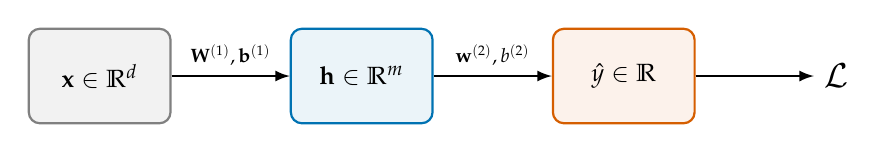
\begin{tikzpicture}[
    layer/.style={rectangle, draw=blue, thick, rounded corners, minimum height=1.2cm, minimum width=1.8cm, fill=blue!8, font=\small},
    >=latex
]
    \node[layer, fill=gray!10, draw=gray] (input) {$\vx \in \R^d$};
    \node[layer, right=1.5cm of input] (h1) {$\vh \in \R^m$};
    \node[layer, fill=red!8, draw=red, right=1.5cm of h1] (out) {$\hat{y} \in \R$};
    \node[right=1.5cm of out, font=\large] (L) {$\mathcal{L}$};

    \draw[->, thick] (input) -- node[above, font=\scriptsize] {$\vW^{(1)}, \vb^{(1)}$} (h1);
    \draw[->, thick] (h1) -- node[above, font=\scriptsize] {$\vw^{(2)}, b^{(2)}$} (out);
    \draw[->, thick] (out) -- (L);
\end{tikzpicture}
\end{center}

\textbf{Forward pass equations:}
\begin{align*}
    \vz^{(1)} &= \vW^{(1)}\vx + \vb^{(1)} && \vz^{(1)} \in \R^m \quad \text{(pre-activation)} \\
    \vh &= \sigma(\vz^{(1)}) && \vh \in \R^m \quad \text{(activation)} \\
    z^{(2)} &= (\vw^{(2)})^\top \vh + b^{(2)} && z^{(2)} \in \R \quad \text{(output logit)} \\
    \hat{y} &= z^{(2)} && \text{(for regression, no final activation)} \\
    \mathcal{L} &= (y - \hat{y})^2 && \text{(MSE loss)}
\end{align*}

\vspace{4pt}
\textbf{Goal:} Compute $\pd{\mathcal{L}}{\vW^{(1)}}$, $\pd{\mathcal{L}}{\vb^{(1)}}$, $\pd{\mathcal{L}}{\vw^{(2)}}$, $\pd{\mathcal{L}}{b^{(2)}}$.
\end{frame}

% ---- Output Layer Gradients ----
\begin{frame}
\frametitle{Backpropagation Step 1: Output Layer Gradients}

\textbf{Start from the loss} and work backward.

\vspace{6pt}
\textbf{Step 1a:} Gradient of loss w.r.t.\ output:
\[
    \pd{\mathcal{L}}{\hat{y}} = \pd{}{\hat{y}}(y - \hat{y})^2 = -2(y - \hat{y})
\]

Since $\hat{y} = z^{(2)}$: \quad $\pd{\mathcal{L}}{z^{(2)}} = -2(y - \hat{y})$. \quad Define $\textcolor{red}{\delta^{(2)} \equiv \pd{\mathcal{L}}{z^{(2)}} = -2(y - \hat{y})}$.

\vspace{8pt}
\textbf{Step 1b:} Gradient w.r.t.\ output layer parameters:
\[
    z^{(2)} = \sum_{j=1}^{m} w_j^{(2)} h_j + b^{(2)}
\]

\[
    \pd{\mathcal{L}}{w_j^{(2)}} = \delta^{(2)} \cdot \pd{z^{(2)}}{w_j^{(2)}} = \textcolor{red}{\delta^{(2)} \cdot h_j} \qquad \Rightarrow \qquad \pd{\mathcal{L}}{\vw^{(2)}} = \delta^{(2)} \cdot \vh
\]

\[
    \pd{\mathcal{L}}{b^{(2)}} = \textcolor{red}{\delta^{(2)}}
\]
\end{frame}

% ---- Hidden Layer Gradients ----
\begin{frame}
\frametitle{Backpropagation Step 2: Hidden Layer Gradients}

\textbf{Step 2a:} Propagate error back to hidden layer. Using chain rule:
\[
    \pd{\mathcal{L}}{h_j} = \pd{\mathcal{L}}{z^{(2)}} \cdot \pd{z^{(2)}}{h_j} = \delta^{(2)} \cdot w_j^{(2)}
\]

\textbf{Step 2b:} Pass through the activation function:
\[
    \pd{\mathcal{L}}{z_j^{(1)}} = \pd{\mathcal{L}}{h_j} \cdot \pd{h_j}{z_j^{(1)}} = \delta^{(2)} \cdot w_j^{(2)} \cdot \sigma'(z_j^{(1)})
\]

Define $\textcolor{red}{\delta_j^{(1)} \equiv \delta^{(2)} \cdot w_j^{(2)} \cdot \sigma'(z_j^{(1)})}$.

\vspace{8pt}
\textbf{Step 2c:} Gradient w.r.t.\ hidden layer parameters:
\[
    z_j^{(1)} = \sum_{k=1}^{d} W_{jk}^{(1)} x_k + b_j^{(1)}
\]

\[
    \pd{\mathcal{L}}{W_{jk}^{(1)}} = \delta_j^{(1)} \cdot x_k \qquad \Rightarrow \qquad \textcolor{red}{\pd{\mathcal{L}}{\vW^{(1)}} = \bm{\delta}^{(1)} \vx^\top}
\]

\[
    \pd{\mathcal{L}}{b_j^{(1)}} = \textcolor{red}{\delta_j^{(1)}}
\]
\end{frame}

% ---- General Backprop Formula ----
\begin{frame}
\frametitle{The General Backpropagation Formula}

Define the \textbf{error signal} at layer $l$: \quad $\bm{\delta}^{(l)} \equiv \pd{\mathcal{L}}{\vz^{(l)}}$

\vspace{6pt}
\begin{tikzpicture}
\node [mybox] (box){%
    \begin{minipage}{0.93\textwidth}
    \vspace{-4pt}
    \textbf{Output layer} ($l = L$): \quad $\bm{\delta}^{(L)} = \pd{\mathcal{L}}{\hat{\vy}} \odot \sigma'(\vz^{(L)})$

    \vspace{6pt}
    \textbf{Hidden layers} ($l = L{-}1, \ldots, 1$): \quad $\bm{\delta}^{(l)} = \left[(\vW^{(l+1)})^\top \bm{\delta}^{(l+1)}\right] \odot \sigma'(\vz^{(l)})$

    \vspace{6pt}
    \textbf{Parameter gradients:} \quad $\pd{\mathcal{L}}{\vW^{(l)}} = \bm{\delta}^{(l)} (\vh^{(l-1)})^\top$ \qquad $\pd{\mathcal{L}}{\vb^{(l)}} = \bm{\delta}^{(l)}$
    \vspace{2pt}
    \end{minipage}
};
\node[fancytitle, right=10pt] at (box.north west) {Backpropagation Equations};
\end{tikzpicture}

\vspace{8pt}
Here $\odot$ denotes element-wise (Hadamard) product and $\vh^{(0)} = \vx$.

\vspace{4pt}
\textbf{Intuition:} The error at layer $l$ is the error from layer $l{+}1$ projected back through $\vW^{(l+1)}$, scaled by how sensitive the activation was ($\sigma'$).
\end{frame}

% ---- Backprop Summary Diagram ----
\begin{frame}
\frametitle{Backpropagation: Visual Summary}

\begin{center}
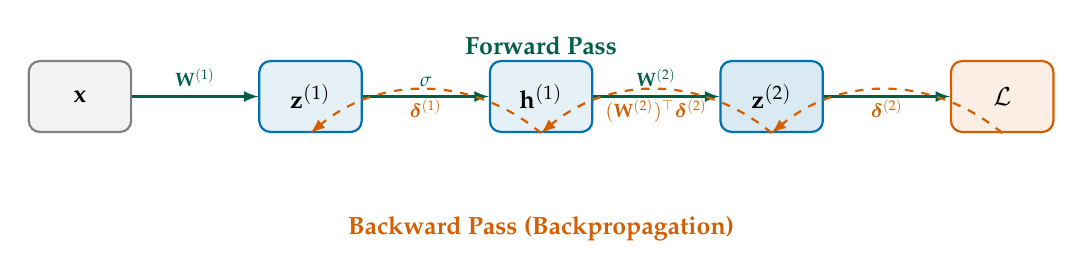
\begin{tikzpicture}[
    layer/.style={rectangle, draw, thick, rounded corners, minimum height=0.9cm, minimum width=1.3cm, font=\small},
    >=latex, node distance=1.6cm
]
    % Layers
    \node[layer, draw=gray, fill=gray!10] (x) {$\vx$};
    \node[layer, draw=blue, fill=blue!10, right=of x] (z1) {$\vz^{(1)}$};
    \node[layer, draw=blue, fill=blue!10, right=of z1] (h1) {$\vh^{(1)}$};
    \node[layer, draw=blue, fill=blue!15, right=of h1] (z2) {$\vz^{(2)}$};
    \node[layer, draw=red, fill=red!10, right=of z2] (L) {$\mathcal{L}$};

    % Forward arrows (on top)
    \draw[->, thick, green!60!black] (x) -- node[above, font=\scriptsize] {$\vW^{(1)}$} (z1);
    \draw[->, thick, green!60!black] (z1) -- node[above, font=\scriptsize] {$\sigma$} (h1);
    \draw[->, thick, green!60!black] (h1) -- node[above, font=\scriptsize] {$\vW^{(2)}$} (z2);
    \draw[->, thick, green!60!black] (z2) -- (L);

    % Backward arrows (below, well separated)
    \draw[->, thick, red, dashed] (L.south) to[bend right=40] node[below, font=\scriptsize, text=red] {$\bm{\delta}^{(2)}$} (z2.south);
    \draw[->, thick, red, dashed] (z2.south) to[bend right=40] node[below, font=\scriptsize, text=red] {$(\vW^{(2)})^\top\bm{\delta}^{(2)}$} (h1.south);
    \draw[->, thick, red, dashed] (h1.south) to[bend right=40] node[below, font=\scriptsize, text=red] {$\bm{\delta}^{(1)}$} (z1.south);

    % Labels
    \node[above=0.4cm, font=\small\bfseries, text=green!60!black] at ($(z1)!0.5!(z2)$) {Forward Pass};
    \node[below=1.4cm, font=\small\bfseries, text=red] at ($(z1)!0.5!(z2)$) {Backward Pass (Backpropagation)};
\end{tikzpicture}
\end{center}

\vspace{6pt}
\textbf{Algorithm:}
\begin{enumerate}
    \item \textcolor{green!60!black}{\textbf{Forward:}} Compute all $\vz^{(l)}$, $\vh^{(l)}$, and $\mathcal{L}$ (save intermediate values).
    \item \textcolor{red}{\textbf{Backward:}} Compute $\bm{\delta}^{(L)}, \bm{\delta}^{(L-1)}, \ldots, \bm{\delta}^{(1)}$ using the recursion.
    \item \textbf{Update:} $\vW^{(l)} \leftarrow \vW^{(l)} - \alpha \, \bm{\delta}^{(l)}(\vh^{(l-1)})^\top$ for all $l$.
\end{enumerate}
\end{frame}

% ---- Numerical Example ----
\begin{frame}
\frametitle{Backpropagation: Numerical Example (Part 1)}

\textbf{Network:} 1 input $\to$ 1 hidden (sigmoid) $\to$ 1 output (linear). MSE loss.

\vspace{4pt}
\textbf{Parameters:} $w^{(1)} = 0.5$, $b^{(1)} = 0.1$, $w^{(2)} = -0.3$, $b^{(2)} = 0.2$

\textbf{Data:} $x = 2.0$, $y = 1.0$. \qquad \textbf{Learning rate:} $\alpha = 0.1$.

\vspace{8pt}
\textbf{Forward pass:}
\begin{align*}
    z^{(1)} &= w^{(1)} x + b^{(1)} = 0.5 \cdot 2.0 + 0.1 = 1.1 \\[4pt]
    h &= \sigma(z^{(1)}) = \sigma(1.1) = \frac{1}{1 + e^{-1.1}} = 0.7503 \\[4pt]
    z^{(2)} &= w^{(2)} h + b^{(2)} = -0.3 \cdot 0.7503 + 0.2 = -0.0251 \\[4pt]
    \hat{y} &= z^{(2)} = -0.0251 \\[4pt]
    \mathcal{L} &= (y - \hat{y})^2 = (1.0 - (-0.0251))^2 = (1.0251)^2 = 1.0508
\end{align*}
\end{frame}

% ---- Numerical Example Part 2 ----
\begin{frame}
\frametitle{Backpropagation: Numerical Example (Part 2)}

\textbf{Backward pass:}

\vspace{4pt}
\textbf{Step 1:} Error at output:
\[
    \delta^{(2)} = \pd{\mathcal{L}}{z^{(2)}} = -2(y - \hat{y}) = -2(1.0 - (-0.0251)) = \textcolor{red}{-2.0502}
\]

\textbf{Step 2:} Gradients for output layer:
\[
    \pd{\mathcal{L}}{w^{(2)}} = \delta^{(2)} \cdot h = -2.0502 \cdot 0.7503 = \textcolor{red}{-1.5383}
\]
\[
    \pd{\mathcal{L}}{b^{(2)}} = \delta^{(2)} = \textcolor{red}{-2.0502}
\]

\textbf{Step 3:} Error at hidden layer:
\[
    \delta^{(1)} = \delta^{(2)} \cdot w^{(2)} \cdot \sigma'(z^{(1)}) = -2.0502 \cdot (-0.3) \cdot 0.7503 \cdot (1 - 0.7503) = \textcolor{red}{0.1154}
\]

\textbf{Step 4:} Gradients for hidden layer:
\[
    \pd{\mathcal{L}}{w^{(1)}} = \delta^{(1)} \cdot x = 0.1154 \cdot 2.0 = \textcolor{red}{0.2307}
\]
\[
    \pd{\mathcal{L}}{b^{(1)}} = \delta^{(1)} = \textcolor{red}{0.1154}
\]
\end{frame}

% ---- Numerical Example Part 3 ----
\begin{frame}
\frametitle{Backpropagation: Numerical Example (Part 3)}

\textbf{Parameter update} with learning rate $\alpha = 0.1$: \quad $\theta_{\text{new}} = \theta_{\text{old}} - \alpha \cdot \text{grad}$

\vspace{4pt}
\renewcommand{\arraystretch}{1.3}
\begin{center}
{\small
\begin{tabular}{lccc}
\toprule
\textbf{Parameter} & \textbf{Old} & \textbf{Gradient} & \textbf{New} \\
\midrule
$w^{(2)}$ & $-0.3000$ & $-1.5383$ & $-0.1462$ \\
$b^{(2)}$ & $0.2000$ & $-2.0502$ & $0.4050$ \\
$w^{(1)}$ & $0.5000$ & $0.2307$ & $0.4769$ \\
$b^{(1)}$ & $0.1000$ & $0.1154$ & $0.0885$ \\
\bottomrule
\end{tabular}
}
\end{center}

\vspace{4pt}
\textbf{Verify:} Forward pass with new params $\to$ $\hat{y}_{\text{new}} = 0.2969$
\[
    \mathcal{L}_{\text{new}} = (1.0 - 0.2969)^2 = 0.4946 \quad \textcolor{green}{\text{(down from 1.0508!} \; \checkmark\text{)}}
\]

\textbf{One gradient step reduced the loss by 53\%.} Repeat this process thousands of times to train the network.
\end{frame}

% ---- Matrix Calculus ----
\begin{frame}
\frametitle{Vector and Matrix Calculus Notation}

In practice, we work with \textbf{matrices}, not individual weights.

\vspace{6pt}
\textbf{Key identities} (for layer $l$):

\vspace{4pt}
If $\vz^{(l)} = \vW^{(l)}\vh^{(l-1)} + \vb^{(l)}$, then:

\begin{align*}
    \pd{\mathcal{L}}{\vW^{(l)}} &= \bm{\delta}^{(l)} \cdot (\vh^{(l-1)})^\top && \in \R^{m^{(l)} \times m^{(l-1)}} \\[8pt]
    \pd{\mathcal{L}}{\vb^{(l)}} &= \bm{\delta}^{(l)} && \in \R^{m^{(l)}} \\[8pt]
    \pd{\mathcal{L}}{\vh^{(l-1)}} &= (\vW^{(l)})^\top \bm{\delta}^{(l)} && \in \R^{m^{(l-1)}}
\end{align*}

\vspace{6pt}
\textbf{Why outer product?} Each $\delta_j^{(l)}$ pairs with each $h_k^{(l-1)}$:
\[
    \pd{\mathcal{L}}{W_{jk}^{(l)}} = \delta_j^{(l)} \cdot h_k^{(l-1)} \quad \Rightarrow \quad \pd{\mathcal{L}}{\vW^{(l)}} = \bm{\delta}^{(l)} (\vh^{(l-1)})^\top
\]

\vspace{4pt}
\textcolor{red}{Same gradient shape as the parameter:} $\pd{\mathcal{L}}{\vW^{(l)}}$ has the same dimensions as $\vW^{(l)}$.
\end{frame}

% ---- Backprop Complexity ----
\begin{frame}
\frametitle{Computational Cost of Backpropagation}

\begin{wideitemize}
    \item \textbf{Forward pass cost:} $O\!\left(\sum_{l=1}^{L} m^{(l)} \cdot m^{(l-1)}\right)$ \quad (matrix-vector products).

    \item \textbf{Backward pass cost:} same order as forward pass!
    \begin{itemize}
        \item Each layer: one matrix-vector product $(\vW^{(l)})^\top \bm{\delta}^{(l)}$.
        \item Plus one outer product $\bm{\delta}^{(l)}(\vh^{(l-1)})^\top$.
    \end{itemize}

    \item \textbf{Memory cost:} must store all intermediate $\vz^{(l)}$, $\vh^{(l)}$ during forward pass.

    \item \textbf{Total:} Backpropagation is roughly \textbf{2x the cost of the forward pass}.
\end{wideitemize}

\vspace{8pt}
\begin{tikzpicture}
\node [mybox] (box){%
    \begin{minipage}{0.93\textwidth}
    \textbf{Before backpropagation} (1986): computing gradients for a network with $P$ parameters required $O(P)$ separate forward passes (one per parameter).

    \textbf{With backpropagation:} \textcolor{red}{all gradients in one backward pass} --- $O(1)$ relative to forward pass.
    \end{minipage}
};
\node[fancytitle, right=10pt] at (box.north west) {Historical Significance};
\end{tikzpicture}
\end{frame}


% ============================================================
\section{Gradient Descent Variants}
% ============================================================

\begin{transitionframe}
\begin{center}
{\Huge \textbf{Gradient Descent Variants}}
\end{center}
\end{transitionframe}

% ---- Batch GD ----
\begin{frame}
\frametitle{Batch Gradient Descent}

\textbf{Full batch gradient descent} uses \textbf{all} $N$ samples to compute the gradient:
\[
    \vw \leftarrow \vw - \alpha \cdot \frac{1}{N}\sum_{i=1}^{N} \nabla_{\vw}\ell(\vx_i, y_i; \vw)
\]

\vspace{6pt}
\textbf{Pros:}
\begin{itemize}
    \item Stable convergence, low noise.
    \item Exact gradient direction.
\end{itemize}

\vspace{4pt}
\textbf{Cons:}
\begin{itemize}
    \item Requires loading \textbf{entire dataset} into memory.
    \item Very slow for large $N$ (one update per epoch).
    \item Can get stuck in local minima (smooth trajectory).
\end{itemize}

\vspace{6pt}
\textbf{Not practical} when $N$ is large (e.g., ImageNet: $N = 1.2$ million).
\end{frame}

% ---- SGD ----
\begin{frame}
\frametitle{Stochastic Gradient Descent (SGD)}

\textbf{SGD} uses a \textbf{single random sample} per update:
\[
    \vw \leftarrow \vw - \alpha \cdot \nabla_{\vw}\ell(\vx_i, y_i; \vw) \qquad \text{where $i$ is sampled randomly}
\]

\vspace{6pt}
\begin{columns}[T]
\begin{column}{0.48\textwidth}
\textbf{Pros:}
\begin{itemize}
    \item Very fast updates.
    \item Can escape shallow local minima (noise helps!).
    \item Low memory requirement.
\end{itemize}
\end{column}

\begin{column}{0.48\textwidth}
\textbf{Cons:}
\begin{itemize}
    \item Very noisy gradient estimate.
    \item Oscillates around minimum.
    \item May never converge exactly.
\end{itemize}
\end{column}
\end{columns}

\vspace{8pt}
\textbf{Key insight:} SGD's gradient is an \textbf{unbiased estimate} of the true gradient:
\[
    \E_i\left[\nabla_{\vw}\ell(\vx_i, y_i; \vw)\right] = \frac{1}{N}\sum_{i=1}^{N}\nabla_{\vw}\ell(\vx_i, y_i; \vw) = \nabla_{\vw}\mathcal{L}(\vw)
\]
\end{frame}

% ---- Mini-Batch SGD ----
\begin{frame}
\frametitle{Mini-Batch SGD: The Best of Both Worlds}

\textbf{Mini-batch SGD} uses a random subset $\mathcal{B} \subset \{1, \ldots, N\}$ of size $B$:
\[
    \vw \leftarrow \vw - \alpha \cdot \frac{1}{B}\sum_{i \in \mathcal{B}} \nabla_{\vw}\ell(\vx_i, y_i; \vw)
\]

\vspace{6pt}
\renewcommand{\arraystretch}{1.4}
\begin{center}
\begin{tabular}{llll}
\toprule
\textbf{Method} & \textbf{Batch size} & \textbf{Noise} & \textbf{Speed} \\
\midrule
Batch GD & $B = N$ & None & Slow \\
SGD & $B = 1$ & High & Fast \\
\textcolor{red}{Mini-batch SGD} & \textcolor{red}{$B = 32, 64, 128, 256$} & \textcolor{red}{Moderate} & \textcolor{red}{Fast} \\
\bottomrule
\end{tabular}
\end{center}

\vspace{4pt}
\textbf{Why mini-batches work so well:}
\begin{itemize}
    \item GPUs are optimized for \textbf{parallel matrix operations} --- processing 32 samples is almost as fast as 1.
    \item Noise is reduced by factor $\frac{1}{\sqrt{B}}$ vs.\ pure SGD.
    \item Typical batch sizes: \textbf{32, 64, 128, 256} (powers of 2 for GPU efficiency).
\end{itemize}
\end{frame}

% ---- Epoch and Iterations ----
\begin{frame}
\frametitle{Epochs, Iterations, and Batch Size}

\begin{tikzpicture}
\node [mybox] (box){%
    \begin{minipage}{0.93\textwidth}
    \begin{itemize}
        \item \textbf{Epoch:} one complete pass through the entire dataset.
        \item \textbf{Iteration:} one parameter update (= one mini-batch).
        \item \textbf{Iterations per epoch:} $\lceil N / B \rceil$.
    \end{itemize}
    \end{minipage}
};
\node[fancytitle, right=10pt] at (box.north west) {Terminology};
\end{tikzpicture}

\vspace{8pt}
\textbf{Example:} $N = 10{,}000$ training samples, batch size $B = 100$:
\begin{itemize}
    \item Iterations per epoch: $10{,}000 / 100 = 100$.
    \item If we train for 50 epochs: $50 \times 100 = 5{,}000$ total parameter updates.
\end{itemize}

\vspace{8pt}
\textbf{Training recipe:}
\begin{enumerate}
    \item Shuffle the dataset.
    \item Split into mini-batches of size $B$.
    \item For each mini-batch: forward $\to$ loss $\to$ backward $\to$ update.
    \item Repeat for multiple epochs.
\end{enumerate}
\end{frame}

% ---- Momentum ----
\begin{frame}
\frametitle{SGD with Momentum}

Pure SGD oscillates due to noisy gradients. \textbf{Momentum} smooths the trajectory:

\begin{tikzpicture}
\node [mybox] (box){%
    \begin{minipage}{0.93\textwidth}
    \[
        \mathbf{v}_t = \beta \, \mathbf{v}_{t-1} + \nabla_{\vw}\mathcal{L}(\vw_t) \qquad \vw_{t+1} = \vw_t - \alpha \, \mathbf{v}_t
    \]
    where $\beta \in [0, 1)$ is the momentum coefficient (typically $\beta = 0.9$).
    \end{minipage}
};
\node[fancytitle, right=10pt] at (box.north west) {Momentum Update};
\end{tikzpicture}

\vspace{6pt}
\textbf{Intuition:} Think of a ball rolling down a hill. Momentum accumulates past gradients, so the ball ``rolls through'' small bumps instead of getting stuck.

\vspace{6pt}
\begin{columns}[T]
\begin{column}{0.48\textwidth}
\centering
\textcolor{blue}{\textbf{Without momentum}}

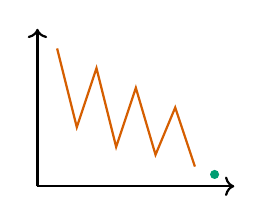
\begin{tikzpicture}[scale=0.5]
    \draw[thick, ->] (0,0) -- (5,0);
    \draw[thick, ->] (0,0) -- (0,4);
    \draw[thick, red] (0.5, 3.5) -- (1, 1.5) -- (1.5, 3) -- (2, 1) -- (2.5, 2.5) -- (3, 0.8) -- (3.5, 2) -- (4, 0.5);
    \draw[fill=green, green] (4.5, 0.3) circle (0.1);
\end{tikzpicture}

{\small Oscillates, slow convergence.}
\end{column}

\begin{column}{0.48\textwidth}
\centering
\textcolor{blue}{\textbf{With momentum}}

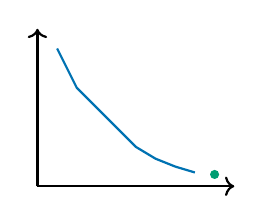
\begin{tikzpicture}[scale=0.5]
    \draw[thick, ->] (0,0) -- (5,0);
    \draw[thick, ->] (0,0) -- (0,4);
    \draw[thick, blue] (0.5, 3.5) -- (1, 2.5) -- (1.5, 2) -- (2, 1.5) -- (2.5, 1) -- (3, 0.7) -- (3.5, 0.5) -- (4, 0.35);
    \draw[fill=green, green] (4.5, 0.3) circle (0.1);
\end{tikzpicture}

{\small Smoother, faster convergence.}
\end{column}
\end{columns}
\end{frame}


% ============================================================
\section{PyTorch Implementation}
% ============================================================

\begin{transitionframe}
\begin{center}
{\Huge \textbf{PyTorch Implementation}}
\end{center}
\end{transitionframe}

% ---- PyTorch Backprop ----
\begin{frame}[fragile]
\frametitle{Backpropagation in PyTorch: Under the Hood}

\textbf{PyTorch does backpropagation automatically} via \texttt{autograd}.

\vspace{4pt}
\begin{lstlisting}
import torch
import torch.nn as nn

# 2-layer network: 3 inputs -> 4 hidden (ReLU) -> 1 output
model = nn.Sequential(
    nn.Linear(3, 4),     # W1: 4x3, b1: 4   -> 16 params
    nn.ReLU(),
    nn.Linear(4, 1),     # W2: 1x4, b2: 1   -> 5 params
)                        # Total: 21 parameters

# Forward pass
x = torch.randn(1, 3)        # 1 sample, 3 features
y_true = torch.tensor([[1.0]])
y_pred = model(x)

# Compute loss
loss = nn.MSELoss()(y_pred, y_true)

# Backward pass -- computes ALL gradients automatically!
loss.backward()

# Inspect gradients
for name, param in model.named_parameters():
    print(f"{name}: grad shape = {param.grad.shape}")
\end{lstlisting}
\end{frame}

% ---- Full Training ----
\begin{frame}[fragile]
\frametitle{Full Training Example: Economic Data}

\begin{lstlisting}
import torch
import torch.nn as nn
from torch.utils.data import DataLoader, TensorDataset

# Simulated economic data: 3 features -> predict outcome
X = torch.randn(1000, 3)             # 1000 samples, 3 features
y = (2*X[:,0] - X[:,1] + 0.5*X[:,2] + torch.randn(1000)*0.1).unsqueeze(1)

# DataLoader for mini-batch SGD
dataset = TensorDataset(X, y)
loader = DataLoader(dataset, batch_size=32, shuffle=True)

# Model, loss, optimizer
model = nn.Sequential(nn.Linear(3, 16), nn.ReLU(),
                      nn.Linear(16, 8), nn.ReLU(),
                      nn.Linear(8, 1))
criterion = nn.MSELoss()
optimizer = torch.optim.SGD(model.parameters(), lr=0.01, momentum=0.9)

# Training loop
for epoch in range(50):
    for X_batch, y_batch in loader:
        y_pred = model(X_batch)         # Forward
        loss = criterion(y_pred, y_batch)
        optimizer.zero_grad()           # Reset gradients
        loss.backward()                 # Backward (backpropagation!)
        optimizer.step()                # Update: w <- w - alpha * grad
\end{lstlisting}
\end{frame}

% ---- Visualizing Loss ----
\begin{frame}[fragile]
\frametitle{Visualizing the Training Loss}

\begin{lstlisting}
import matplotlib.pyplot as plt

losses = []
for epoch in range(100):
    epoch_loss = 0
    for X_batch, y_batch in loader:
        y_pred = model(X_batch)
        loss = criterion(y_pred, y_batch)
        optimizer.zero_grad()
        loss.backward()
        optimizer.step()
        epoch_loss += loss.item()
    losses.append(epoch_loss / len(loader))

plt.plot(losses)
plt.xlabel('Epoch')
plt.ylabel('MSE Loss')
plt.title('Training Loss Curve')
plt.grid(True)
plt.show()
\end{lstlisting}

\vspace{4pt}
\textbf{What to look for:}
\begin{itemize}
    \item Loss should \textbf{decrease} over epochs.
    \item If it oscillates wildly: learning rate is too large.
    \item If it decreases very slowly: learning rate is too small.
\end{itemize}
\end{frame}


% ============================================================
\section{Summary and Next Steps}
% ============================================================

\begin{transitionframe}
\begin{center}
{\Huge \textbf{Summary \& Next Steps}}
\end{center}
\end{transitionframe}

% ---- Summary ----
\begin{frame}
\frametitle{Lecture 2 Summary}

\begin{enumerate}
    \item \textbf{Activation function derivatives} are critical for backprop. Sigmoid: $\sigma' = \sigma(1-\sigma)$. ReLU: $\sigma' = \mathbbm{1}[z > 0]$.

    \item \textbf{Vanishing gradients:} sigmoid derivative $\leq 0.25$ causes exponential decay in deep nets. ReLU solves this.

    \item \textbf{Softmax} extends binary classification to $K$ classes: $\hat{y}_k = \frac{e^{z_k}}{\sum_j e^{z_j}}$.

    \item \textbf{Cross-entropy + softmax/sigmoid} gives gradient $\pd{\mathcal{L}}{z_i} = \hat{y}_i - y_i$.

    \item \textbf{Backpropagation} = chain rule applied layer by layer:
    \[
        \bm{\delta}^{(l)} = [(\vW^{(l+1)})^\top \bm{\delta}^{(l+1)}] \odot \sigma'(\vz^{(l)}) \qquad \pd{\mathcal{L}}{\vW^{(l)}} = \bm{\delta}^{(l)}(\vh^{(l-1)})^\top
    \]

    \item \textbf{Mini-batch SGD} with momentum is the standard optimizer. Typical $B = 32$--$256$.
\end{enumerate}
\end{frame}

% ---- Next Lecture ----
\begin{frame}
\frametitle{Next Lecture: SGD, Regularization \& Generalization}

\textbf{Lecture 3} (Monday, April 20):
\begin{wideitemize}
    \item Advanced optimizers: Adam, AdaGrad, RMSProp.
    \item Regularization: L1, L2 (weight decay), dropout.
    \item Batch normalization.
    \item The Universal Approximation Theorem.
    \item Why depth matters more than width.
    \item Practical tips: learning rate schedules, early stopping.
\end{wideitemize}

\vspace{10pt}
\textbf{Recommended reading:}
\begin{itemize}
    \item Goodfellow et al., \textit{Deep Learning}, Chapter 6.5 (Backpropagation), Chapter 8 (Optimization).
    \item Zhang et al., \textit{Dive into Deep Learning}, Chapter 5 (\url{https://d2l.ai}).
\end{itemize}

\vspace{10pt}
\textbf{Homework 1} will be released after Lecture 3 (due Sunday, April 27).

\vspace{6pt}
\begin{center}
\Large \textcolor{blue}{\textbf{Questions?}}
\end{center}
\end{frame}

% ---- References ----
\begin{frame}
\frametitle{References}

\small
\begin{wideitemize}
    \item Goodfellow, I., Bengio, Y., \& Courville, A. (2016). \textit{Deep Learning}. MIT Press. Chapters 6, 8.
    \item Zhang, A., Lipton, Z. C., Li, M., \& Smola, A. J. (2023). \textit{Dive into Deep Learning}. Cambridge University Press.
    \item Rumelhart, D. E., Hinton, G. E., \& Williams, R. J. (1986). Learning representations by back-propagating errors. \textit{Nature}, 323(6088), 533--536.
    \item Glorot, X., \& Bengio, Y. (2010). Understanding the difficulty of training deep feedforward neural networks. \textit{AISTATS}.
    \item Nair, V., \& Hinton, G. E. (2010). Rectified linear units improve restricted Boltzmann machines. \textit{ICML}.
    \item Kingma, D. P., \& Ba, J. (2015). Adam: A method for stochastic optimization. \textit{ICLR}.
\end{wideitemize}
\end{frame}

\end{document}
